\documentclass[11pt]{article}

\usepackage{amsmath,amssymb,amsfonts}
\usepackage{graphicx}
\usepackage{pgfplots}
\usepackage{multicol}
\usepackage{enumitem}


\setlength{\topmargin}{-.5in} \setlength{\textheight}{9.25in}
\setlength{\oddsidemargin}{0in} \setlength{\textwidth}{6.8in}


\begin{document}

\Large


\noindent{\bf Name: \hfill Date: \hfill Exam 2 \hfill Calculus - Hargus}

\medskip\hrule
\vspace{20pt}

\noindent \textbf{Instructions:} Please \textbf{show all work} on the test paper (partial credit may be awarded for correct work, even if your answer is wrong). You may use the back side if you run out of room. Calculators are not allowed, but \textbf{simplify} your answers as much as you can. Cheating of any kind will result in a score of zero.

\vspace{10pt}

\begin{enumerate}[itemsep=30pt]

\item (4 points) True or false?
\begin{enumerate}[itemsep=10pt]
    \item \rule{1cm}{0.4pt} A function $f(x)$ can have at most one derivative function.
    \item \rule{1cm}{0.4pt} A function $f(x)$ can have at most one antiderivative function.
\end{enumerate}

\item (6 points) Label \textbf{all} points of inflection, local minimums, and local maximums. Then, between each of these transition points, label the graph with the sign of $f'(x)$ and $f''(x)$. For example, if $f'(x)>0$ and $f''(x)<0$ for some part of the graph, then write $+-$ next to that part of the graph.
\vspace{10pt}
\begin{center}
\begin{tikzpicture}
\begin{axis}[ xlabel={$x$}, ylabel={$y$}
  ,axis lines=middle
  ,height=7cm
  ,width=12.5cm
  ,samples=1000, grid, thick
  ,domain=-10:10
  ,restrict y to domain=-10:10
  ,axis equal
  ,legend pos=outer north east
  ,xmin=-1.5, xmax=5,
  ,ymin=-0.5, ymax=2.5
  ];
\addplot+[no marks] {((x-1)^2*(x-3)*(x+1)*(x-4)+15)/20};
\end{axis}
\end{tikzpicture}
\end{center}


\item (4 points) If $\lim_{x \to -\infty} f(x) = 3$, what kind of asymptote does $f(x)$ definitely have (circle: \textbf{horizontal} or \textbf{vertical}) and what is the equation for that asymptote's line?
\begin{flushright}
Equation for asymptote: \rule{4cm}{0.4pt}
\end{flushright}

\newpage


\item (12 points) Evaluate the definite integral.
\begin{enumerate}[itemsep=80pt]
    \item $\int_{2}^{3} x^2 dx = $
    \item $\int_{0}^{\pi/2} \cos(x) dx = $
    \item $\int_{1}^{2} \frac{1}{x} dx = $
    \item $\int_{0}^{1} -e^x dx = $
\end{enumerate}
\vspace{60pt}


\item (4 points) Evaluate the following limit. \textbf{Hint:} Find the function $f(x)$ which has a derivative at $x=1$ equal to this limit (remember the limit definition of the derivative), and then find $f'(1)$.

\vspace{10pt}
$\displaystyle{\lim_{x \to 1} \frac{(x^4+x+3) - 5}{x-1} = }$


\newpage


\item (12 points) Evaluate the indefinite integral.
\begin{enumerate}[itemsep=40pt]
    \item $\int x^2 dx = $
    \item $\int -\cos(x) dx = $
    \item $\int -x^{-3} dx = $
    \item $\int (x-3)(x-1) dx = $
    \item $\int 4\sin(2x)dx = $
    \item $\int 5x^4+1dx  =$
    \item $\int e^{2x} dx = $
    \item $\int \frac{2}{x} dx  =$
\end{enumerate}

\vspace{10 mm}

\item (4 points) Suppose that $f'(-1)=0$.  If $f''(3) > 0$, what does the graph of $f(x)$ have at $x=-1$? (circle one answer)
\begin{enumerate}
    \item Maximum
    \item Minimum
    \item Point of inflection
\end{enumerate}


\newpage


\item (12 points) Find the critical points for the function $f(x) = \frac{1}{3}x^3 -x + 1$. Then, find the transition points and draw a sign chart $f'(x)$ and a sign chart for $f''(x)$ showing the intervals where each function is positive or negative. Then, use this information to sketch the graph $f(x)$ below. Label all minimums, maximums, and points of inflection.
\\

\vspace{80 mm}

\vspace{10pt}
\begin{center}
\begin{tikzpicture}
\begin{axis}[ xlabel={$x$}, ylabel={$y$}
  ,axis lines=middle
  ,height=10cm
  ,width=14cm
  ,samples=500, grid, thick
  ,domain=-10:10
  ,restrict y to domain=-10:10
  ,legend pos=outer north east
  ,xmin=-2, xmax=2,
  ,ymin=-5, ymax=5
  ]
\addplot+[no marks] {-10};
\end{axis}
\end{tikzpicture}
\end{center}


\newpage


\item (8 points) Evaluate the limit, if it exists:
\begin{multicols}{2}
\begin{enumerate}[itemsep=50pt]
    \item $\displaystyle{\lim_{x \to -1} x}$
    \item $\displaystyle{\lim_{x \to 3} \frac{x - 3}{x^2 - 2x - 3}}$
    \item $\displaystyle{\lim_{t \to 0} \frac{4^{2t} - 1}{4^t - 1}}$
    \item $\displaystyle{\lim_{x \to \infty} \frac{x^4}{x^2 + 1}}$
\end{enumerate}
\end{multicols}

\vspace{50pt}

\item (4 points) Which Riemann Sum is shown in the graph below approximating the area under the graph on the interval [0, 4]? (circle one answer)
\begin{multicols}{2}
\begin{enumerate}[itemsep=5pt]
    \item $M_{16}$
    \item $R_{3}$
    \item $L_{12}$
    \item $R_{4}$
\end{enumerate}
\end{multicols}

\begin{center}
\begin{tikzpicture}
\begin{axis}[
    xtick={0,4,8,12,16},ytick={0,...,1.5},
    xmax=18,ymax=1.2,ymin=0,xmin=0,
    width=12cm,height=12cm,
    enlargelimits=true,
    axis lines=middle,
    clip=false,
    domain=0:17,
    axis on top
    ]

\addplot [draw=blue, fill=blue!10, ybar interval, samples=13, domain=0:16]
    {1/(x+1)}\closedcycle;
\addplot[smooth, thick,domain=0:17,samples=40]{1/(x+1)};

\end{axis}
\end{tikzpicture}
\end{center}


\newpage


\item (12 points) Find the derivative $f'(x)$:
\begin{enumerate}[itemsep=40pt]
    \item{$f(x) = x^3 + x + 6$}
    \item{$f(x) = 5\sqrt{x}$}
    \item{$f(x) = 3^x$}
    \item{$f(x) = (-x + 5)^4$}
    \item{$f(x) = \displaystyle{\frac{x^2}{e^x}}$}
    \item{$f(x) = \ln(\sin(x))$}
\end{enumerate}

\vspace{20pt}
\item (6 points) Find the \textbf{second derivative} $y''$ for the given $y$:

\begin{enumerate}[itemsep=50pt]
    \item{$y = -x^2 + 2x^3$}
    \item{$y = 4x^{\frac{1}{4}}$}
    \item{$y = e^x \cos(x)$}
\end{enumerate}


\newpage


\item (6 points) Find $\frac{dy}{dx}$ (the derivative of $y$ with respect to $x$) for the following:
\begin{enumerate}[itemsep=70pt]
    \item $x^2 + y^3 = 1$
    \item $x + e^y + y^2 = 3$
\end{enumerate}

\vspace{30pt}

\item (6 points) For the graph below, draw the derivative function $f'(x)$ on the same graph below (does not need to be exact, though x-intercepts and sign ($+$/$-$) should be correct):

\vspace{10pt}
\begin{center}
\begin{tikzpicture}
\begin{axis}[ xlabel={$x$}, ylabel={$y$}
  ,axis lines=middle
  ,height=10cm
  ,width=10cm
  ,samples=1000, grid, thick
  ,domain=-10:10
  ,restrict y to domain=-10:10
  ,axis equal
  ,legend pos=outer north east
  ,xmin=-2, xmax=5,
  ,ymin=-2, ymax=4
  ]
\addplot+[no marks] {(x-3)*(x-3)*(x+1)/5};
\addlegendentry{$f(x)$}
\end{axis}
\end{tikzpicture}
\end{center}


\item \textbf{Extra Credit} (5 points) If $\int_{1}^{4} f(x)dx = 5$ and $\int_{4}^{9} f(x)dx = 3$, then:

$\displaystyle{\int_{1}^{9} (2f(x) + 1)dx} = $


\end{enumerate}

\end{document} 